
% ----------------------------------------------------------------------
\begin{frame}[shrink]%[allowframebreaks]
  \frametitle{Spatially-extended systems : \KS}

  \begin{center}
    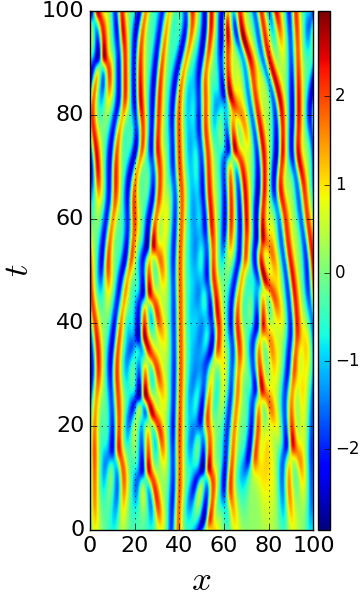
\includegraphics[height=0.6\textheight]{KS_L100N256}
    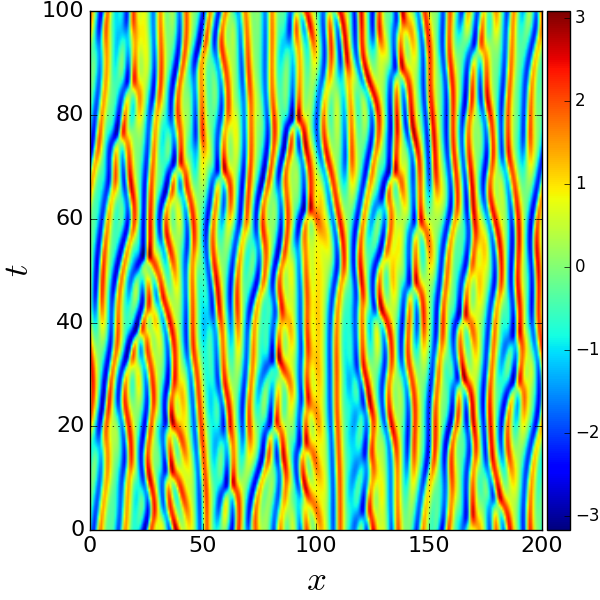
\includegraphics[height=0.6\textheight]{KS_L200N256}
    {
      $u_t+\frac{1}{2}(u^2)_x+u_{xx}+u_{xxxx}=0\,,\; x\in [0,L]$.
    }
  \end{center}

\vfill
  \htbc{\scriptsize
    Recurrent patterns not only show up along the \htr{temporal axis}
    \\
     but also along the \htr{spatial axis}
  }
\end{frame}

% ----------------------------------------------------------------------
\begin{frame}[shrink]%[allowframebreaks]
  \frametitle{\KS\ on a ``minimal domain''}

\bigskip\bigskip

    minimal domain captures essential features observed in large domains

\bigskip

  \begin{center}
    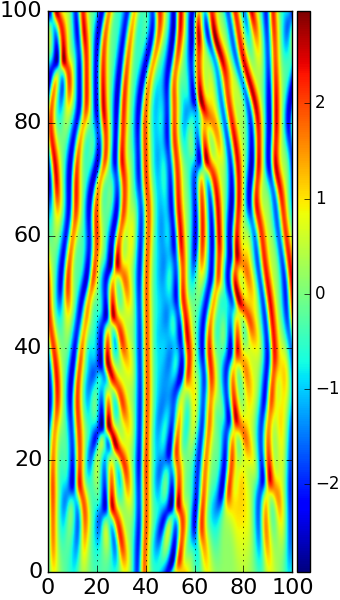
\includegraphics[width=0.182\textwidth]{KS_L100N256NoLable}
    % 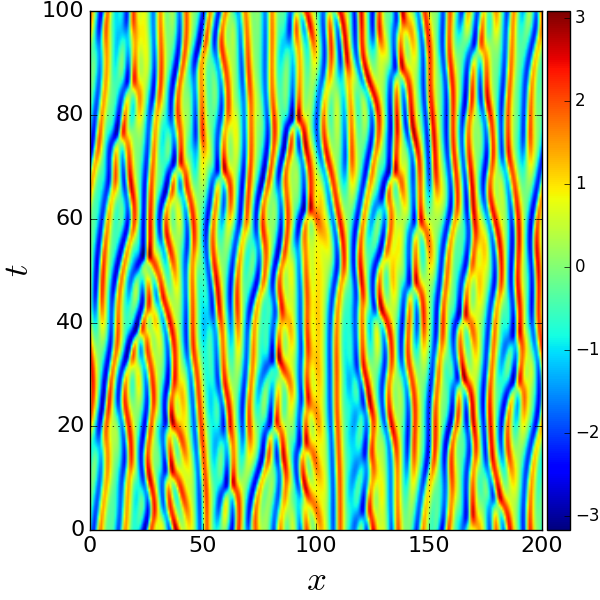
\includegraphics[width=0.6\textwidth]{KS_L200N256}
    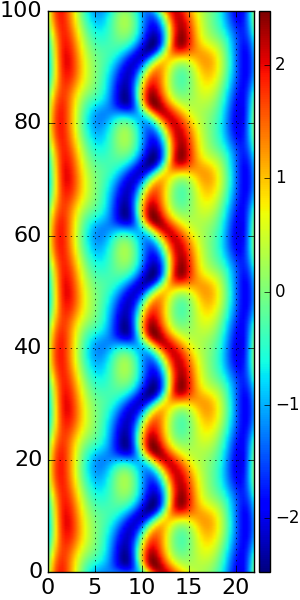
\includegraphics[width=0.16\textwidth]{ksppo1T100NoLabel}
    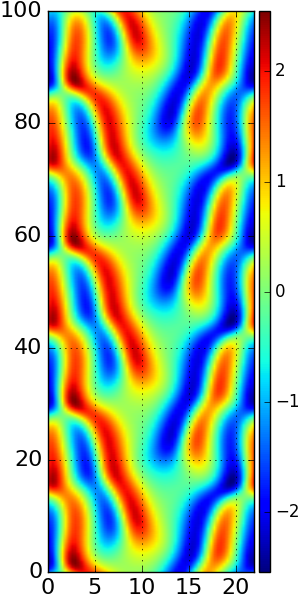
\includegraphics[width=0.16\textwidth]{ksppo2T100NoLabel}
    % 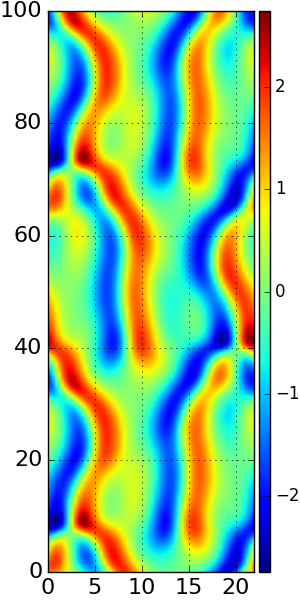
\includegraphics[width=0.16\textwidth]{ksppo3T100NoLabel}
    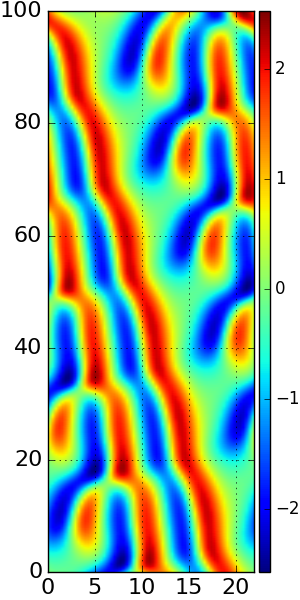
\includegraphics[width=0.16\textwidth]{ksrpo1T100NoLabel}
    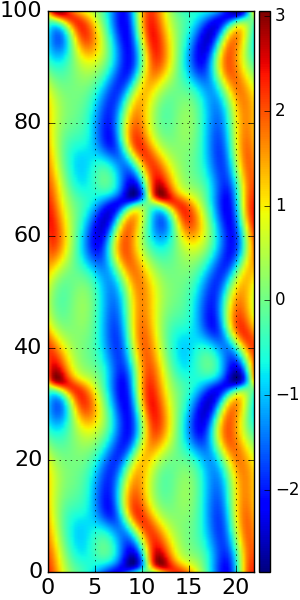
\includegraphics[width=0.16\textwidth]{ksrpo2T100NoLabel}
    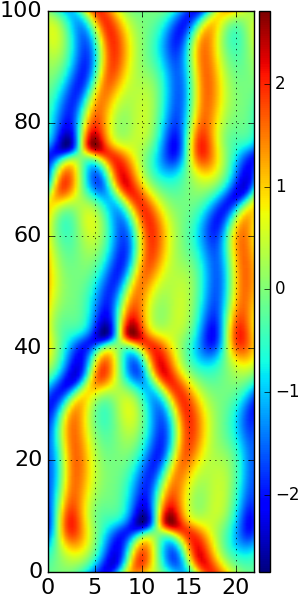
\includegraphics[width=0.16\textwidth]{ksrpo3T100NoLabel}
    {
      horizontally : $x\in [0,L]$

\bigskip

      {\color{blue} (leftmost)  $L = 100$ \qquad (the rest)  $L=22$ }
    }

  \end{center}

\end{frame}
